\documentclass[12pt]{article}
\usepackage[paper=letterpaper,margin=2cm]{geometry}
\usepackage[inline]{enumitem}
\usepackage{enumerate}
\usepackage{amsmath,amsthm,amssymb,amsfonts, color, graphicx,tabularx}
\usepackage{listings} 
\usepackage{mdwlist}
\usepackage{caption, booktabs}
\usepackage{makecell}
\usepackage{fancyhdr}
\usepackage{multicol,paralist}
\usepackage{empheq}
\usepackage[most]{tcolorbox}

\newtcbox{\mymath}[1][]{%
    nobeforeafter, math upper, tcbox raise base,
    enhanced, colframe=blue!30!black,
    colback=blue!30, boxrule=1pt,
    #1}


\title{AP Physics Extra Credit KEY}
\author{Aiden Rosenberg}
\date{November 2022 A.D}
\pagestyle{fancy}
\fancyhf{}
\rhead{\small {© 2022 All Rights Reserved, Aiden Rosenberg}}
\rfoot{Page \thepage}

\begin{document}
\newcommand{\ms}{$\frac{\text{m}}{\text{s}^2}$}

\maketitle

\section{Practice Problems}
\begin{enumerate}
    \item A force of 25 newtons east and a force of 25 newtons west act concurrently on a 5-kilogram cart. Find the acceleration of the cart. 
    
\begin{multicols}{4}
\begin{enumerate}[a)]
\item $1.0$ \ms
\item $0.20$ \ms
\item $5.0$ \ms
\item  $0 $ \ms
\end{enumerate}
\end{multicols}
\begin{empheq}[box=\tcbhighmath]{equation*}
   \Sigma F_x =ma_x= 25N-25N=0N \Longrightarrow a_x=0
\end{empheq}

\item 
A 0.15-kilogram baseball moving at $20$\ms \,  is stopped by a catcher in $0.010$ seconds. The average stopping force of the ball is 
\begin{multicols}{4}
\begin{enumerate}[a)]
\item $3.0 \times 10^{-2}$ N
\item $3.0 \times 10^{0}$ N
\item $3.0 \times 10^{1}$ N
\item $3.0 \times 10^{2}$ N
\end{enumerate}
\end{multicols}
\begin{empheq}[box=\tcbhighmath]{equation*}
  \Sigma F = ma = m\biggr(\frac{v_f-v_0}{t}\biggr)=(0.15kg) \times (-2000\frac{m}{s^2})=-300N
\end{empheq}


\item 
\begin{center}
    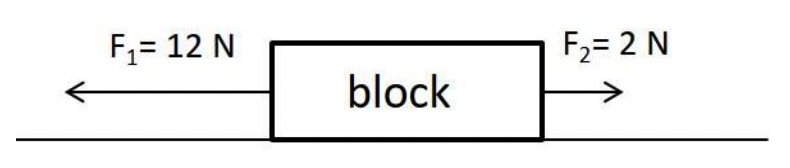
\includegraphics[width=3in]{Screenshot 2022-11-07 at 10.06.01.png}
\end{center}
Two forces $F_1$  and $F_2$, are applied to a block on a friction-less horizontal surface. If the magnitude of the block acceleration is $2.0$\ms, what is the mass of the block?
\begin{multicols}{4}
\begin{enumerate}[a)]
\item 1 kg
\item 5 kg
\item 6 kg
\item 7 kg
\end{enumerate}
\end{multicols}

\begin{empheq}[box=\tcbhighmath]{equation*}
  \Sigma F = ma \Longrightarrow m=\frac{\Sigma F}{a}= \frac{12N-2N}{2\frac{m}{s^2}} = 5kg
\end{empheq}
\newpage
\item A cardboard box of mass $m$ on a wooden floor is represented by the FBD below.
\begin{center}
    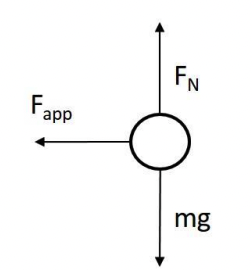
\includegraphics[width=1.5in]{Screenshot 2022-11-07 at 10.06.21.png}
\end{center}
Given the FBD, which of the following expression could be accurately mathematical representations of the box? Chooses all that apply.
\begin{multicols}{4}
\begin{enumerate}[a)]
\item $F_N-mg=ma_x$
\item $-F_{app}=ma_x$
\item $F_N-mg=ma_y$
\item $F_{app}=ma_y$
\end{enumerate}
\end{multicols}

\begin{empheq}[box=\tcbhighmath]{equation*}
  -F_{app}=ma_x \text{ and } F_N-mg=ma_y
\end{empheq}

\item Three objects with differentiating masses are connected by strings and pulled by the right-most string with tension $T_1$ across a frictionless surface as shown to the diagram below. 
\begin{center}
    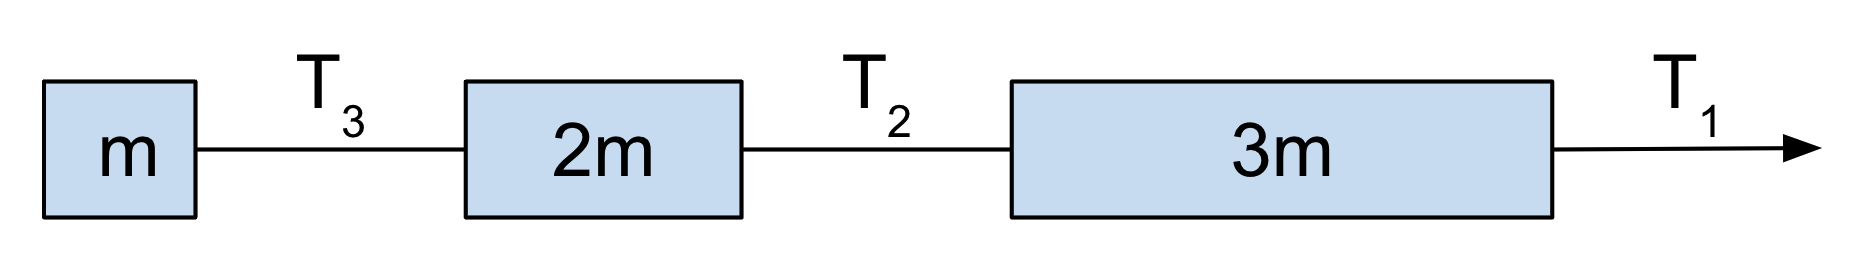
\includegraphics[width=3in]{Screenshot 2022-11-07 at 10.17.18.png}
\end{center}
Which of the following expressions accurately depicts the acceleration of the system? Chose all that apply. 
\begin{multicols}{4}
\begin{enumerate}[a)]
\item $\vec{F}_{net_{X}} = ma_x$
\item $\vec{T}_3=m\vec{a}$
\item $\vec{T}_2-\vec{T}_3=2m\vec{a}$
\item $\vec{T}_1-\vec{T}_2=3m\vec{a}$
\end{enumerate}
\end{multicols}
\begin{empheq}[box=\tcbhighmath]{equation*}
  \textbf{All of the above}
\end{empheq}

\item A 20-newton force due north and a 20-newton force due east act concurrently on an object. The additional force necessary to bring the object into a state of equilibrium is
\begin{multicols}{4}
\begin{enumerate}[a)]
\item 20 N northeast
\item 20 N southwest
\item 28 N northeast
\item 28 N southwest
\end{enumerate}
\end{multicols}

\begin{empheq}[box=\tcbhighmath]{equation*}
  \text{The resultant vector is 28N northeast, $\therefore$  its equilibrium must be  28N Southwest.}
\end{empheq}
\newpage
\item A net force of 10 newtons accelerates an object at 5.0 \ms. What net force would be required to accelerate the same object at 1.0 \ms?
\begin{multicols}{4}
\begin{enumerate}[a)]
\item 1.0 N
\item 2.0 N
\item 5.0 N
\item 50 N
\end{enumerate}
\end{multicols}

\begin{empheq}[box=\tcbhighmath]{equation*}
\begin{aligned}
\Sigma F = ma \Longrightarrow m= \frac{\Sigma F}{a} =\frac{10N}{5 \frac{m}{s^2}}= 2kg \\  \Sigma F = ma = (2kg)(1\frac{m}{s^2})=2N
\end{aligned}
\end{empheq}

\item A 15-kg wagon is pulled to the right across a surface by a tension of 100 newtons at an angle of 30 degrees above a horizontal. A frictional force of 20 newtons to left acts simultaneously. What is the acceleration of the wagon?

\begin{empheq}[box=\tcbhighmath]{equation*}
\begin{aligned}
\Sigma F = ma_x = F_gx - F_f = F_g\cos(30^{\circ}) - 20N = 100\cos(30^{\circ}) - 20N = (50\sqrt{3}-20) N \\ 
a= \frac{\Sigma F}{m}= \frac{(50\sqrt{3}-20)}{15} = \frac{2(5\sqrt{3}-2)}{3} \approx 4.44 \frac{m}{s^2}
\end{aligned}
\end{empheq}

\item A traffic light is suspended by two cables as shown in the diagram. If cable 1 has a tension $T_1=49$ N and $\theta_1 = 30^{\circ}$ and cable 2 has a tension $T_2=85$ N and $\theta_2 = 60^{\circ}$, find the mass of the traffic light. 
\begin{center}
    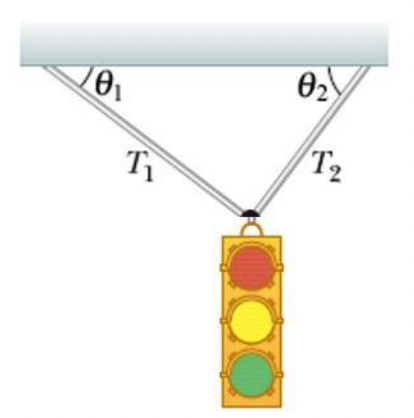
\includegraphics[width=1.5in]{Screenshot 2022-11-07 at 10.37.31.png}
\end{center}

\begin{empheq}[box=\tcbhighmath]{equation*}
\begin{aligned}
\Sigma F_{net_y} = T_1\sin(30^{\circ}) + T_2\sin(60^{\circ}-mg=0)\\
m =\frac{T_1\sin(30^{\circ}) + T_2\sin(60^{\circ}}{g} = \frac{49N\sin(30^{\circ}) + 85N\sin(60^{\circ}}{9.8\frac{m}{s^2}}\\
\Longrightarrow m= 10kg
\end{aligned}
\end{empheq}
\newpage
\item 
The diagram below shoes a block sliding down a plane inclined at angle $\theta$ with the horizontal. 

\begin{center}
    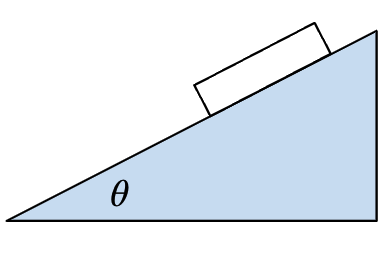
\includegraphics[width=2in]{Screenshot 2022-11-08 at 12.30.49.png}
\end{center}
As the angle $\theta$ is increased the coefficient of kinetic friction between the bottom surface of the incline will
\begin{multicols}{3}
\begin{enumerate}[a)]
\item decrease
\item increases
\item remain the same
\end{enumerate}
\end{multicols}
\begin{empheq}[box=\tcbhighmath]{equation*}
\text{It will remain the same: $\mu_k$ is depended only upon the materials in contact.}
\end{empheq}

\item A force of 50 N to the right is applied to an 4 kg object accelerating it to 10 \ms, 
 on a rough horizontal surface. What is the magnitude of the $F_f$ acting on the object.
\begin{multicols}{4}
\begin{enumerate}[a)]
\item 5.0 N
\item 10 N
\item 20 N
\item 40 N
\end{enumerate}
\end{multicols}

\begin{empheq}[box=\tcbhighmath]{equation*}
\begin{aligned}
F_{net}=ma = F_{app}-F_f\\
F_f = F_{app}-ma\\
F_f= 50N-(4kg)(10\frac{m}{s^2})=10N
\end{aligned}
\end{empheq}

\item Ignatius pulls the handle of a 20-kilogram sled across the yard with a force of 100N at and angle 30 degrees above the horizontal. The yard exerts a friction force of 25N on the sled.
\begin{enumerate}
    \item Find the coefficient of friction between the sled and the yard. 
        \begin{empheq}[box=\tcbhighmath]{equation*}
        \begin{aligned}
            F_{net_y}=ma = 100N\sin(30^{\circ})+F_N-mg=0\\
            F_N=mg-100N\sin(30^{\circ}) = 200N-50N=150N\\
            \mu = \frac{F_f}{F_N}= \frac{25N}{150N} = 0.167
        \end{aligned}
        \end{empheq}
    \item Determine the distance the sled travels if it starts from rest and Ignatius maintains her 100N force for five seconds.  
     \begin{empheq}[box=\tcbhighmath]{equation*}
        \begin{aligned}
            F_{net_x}=ma_x = 100\cos(30^{\circ})-F_f =50\sqrt{3}-25\\
            a_x=\frac{50\sqrt{3}-25}{20kg}=\frac{5(2\sqrt{3}-1)}{4}\\
            \Delta x = v_0t+\frac{1}{2}a_xt^2 = \frac{125(2\sqrt{3}-1)}{8}\approx 38.501 m
        \end{aligned}
    \end{empheq}
\end{enumerate}
\item A 5-kg mass if held at rest on a friction-less $30^{\circ}$ incline by force $F$. What is the magnitude of $F$?
\begin{empheq}[box=\tcbhighmath]{equation*}
        \begin{aligned}
            F_{net}=F-mg_{\parallel}=F-mg\sin(\theta)=0\\
            F=mg\sin(\theta)\\
            F=(5kg)\times(9.8\frac{m}{s^2})\times \sin(30^{\circ})\approx 25.5 N
        \end{aligned}
    \end{empheq}
\item A 10-kg slides down a friction-less $18^{\circ}$ ramp. Find the acceleration of the box, and the time it takes for the box to slide 2 metres down the ramp. 

\begin{empheq}[box=\mymath]{equation*}
        \begin{aligned}
            mg_{\parallel}=mg\sin(\theta)\\
            mg_{\bot}=mg\cos(\theta)
        \end{aligned}
    \end{empheq}
\begin{empheq}[box=\tcbhighmath]{equation*}
        \begin{aligned}
           F_{net}=ma=mg_{\parallel} = mg\sin(\theta)\\
           \Longrightarrow a = g\sin(\theta)= (9.8\frac{m}{s^2})\times \sin(18^{\circ}) = \frac{49(\sqrt{5}-1)}{20} \approx3.028 \frac{m}{s^2}
           \Delta x = v_{0x}t+\frac{1}{2}a_xt^2\\
           t=\sqrt{\frac{2\Delta x}{a}}\approx 1.15 s
        \end{aligned}
    \end{empheq}
\item A block weighting 10 newtons is on a ramp inclined at $30^{\circ}$ to the horizontal. A 3-newton force of friction, $F_f$, acts on the block as it is pulled up the ramp at a constant velocity with force $F$, which is parallel to the ramp. What is the magnitude of force $F$?
\begin{empheq}[box=\tcbhighmath]{equation*}
        \begin{aligned}
           F_{net}=F-F_f-mg\sin(\theta)=0\\
           F=F_f+mg\sin(\theta)=3N+10N\sin(30^{\circ}) = 8N
        \end{aligned}
    \end{empheq}

\item Two masses, $m_1$ and $m_2$, are hanging by a massless string from a friction-less pulley. If $m_1$ is greater than $m_2$, determine the acceleration of the two masses when released from rest. 
\begin{empheq}[box=\mymath]{equation*}
        \begin{aligned}
           m_1g-T=m_1a\\
           T-m_2g=m_2a
        \end{aligned}
    \end{empheq}
\begin{empheq}[box=\tcbhighmath]{equation*}
        \begin{aligned}
             m_1g-m_2a-m_2g=m_1a\\
             m_1g-m_2g=m_1a+m_2a\\
             g((m_1-m_2)=a(m_1+m_2)\\
             a=g\cdot \frac{(m_1-m_2)}{(m_1+m_2)}
        \end{aligned}
    \end{empheq}
\newpage
\item Two masses are hung from a frictionless pulley by a massless spring. If $m_1$ is 5 kg, and $m_2$ is 7 kg, how far will $m_2$ fall in 2 seconds if released from rest. 
\begin{empheq}[box=\tcbhighmath]{equation*}
        \begin{aligned}
            F_{net_y}=m_2g-m_1g=(m_1+m_2)a\\
            a= g \cdot \frac{(m_2-m_1)}{(m_1+m_2)}= (9.8\frac{m}{s^2}) \times \frac{(2kg)}{(12kg)}=\frac{49}{30}\approx 1.63 \frac{m}{s^2}\\
            \Delta y = v_0t+\frac{1}{2}at^2= 0+ \frac{1}{2}(\frac{49}{30})(2)^2 = \frac{49}{15} \approx 3.27 m
        \end{aligned}
    \end{empheq}
    
\item Two masses, $m_1$ and $m_2$, are connected by a light string over a massless pulley as shown. Assuming a frictionless surface, find the acceleration of $m_2$
\begin{empheq}[box=\tcbhighmath]{equation*}
        \begin{aligned}
           F_{net_x}=T=m_1a\\
           F_{net_y}=m_2g-T=m_2a\\
           m_2_g-m_1a=m_2a \Longrightarrow a= g \times \biggr( \frac{m_2}{m_1+m_2} \biggr)
        \end{aligned}
    \end{empheq}

\begin{center}
    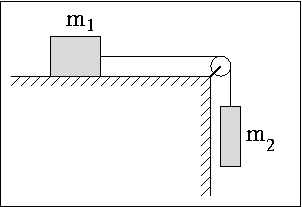
\includegraphics[width=1.5in]{media_d36_d36ac948-3b1e-414d-8e8d-4b93cefb9ce9_phpPqxJSC.png}
\end{center}
\item Identify the physicist in the picture below. 
\begin{center}
    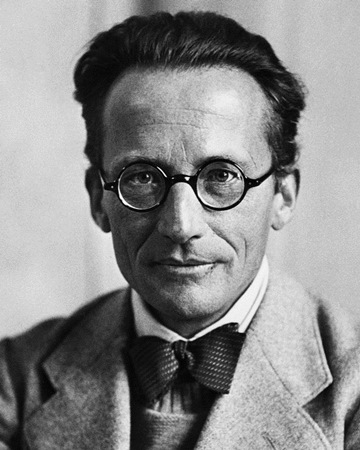
\includegraphics[width=1in]{erwin-schrodinger-medium.jpg}
\end{center}
\begin{empheq}[box=\tcbhighmath]{equation*}
    \textbf{Erwin Schrödinger}
\end{empheq}

\end{enumerate}
\newpage
\section{FRQ Practice}
\begin{enumerate}
    \item (12 points, suggested time 25 minutes)
    \begin{center}
        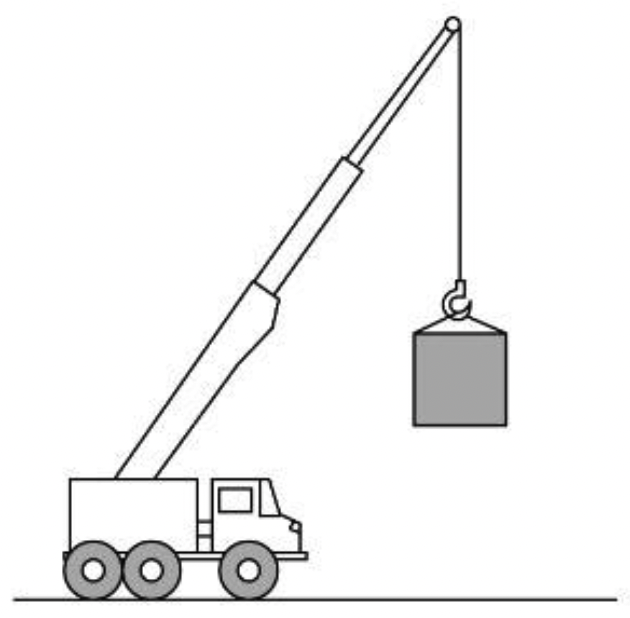
\includegraphics[width=2in]{Screenshot 2022-11-06 at 22.18.57.png}
    \end{center}
    A crane and box are initially at rest. At time $t=0$, the crane begins to drive forward at a constant speed of $0.5 \frac{\text{m}}{\text{s}}$ , while also lifting the box with an upward acceleration of 1 \ms. The box does not swing by the crane. 
    \begin{enumerate}
        \item Draw a FBD, that represents the forces acting on the box.
        \item Using graph-paper sketch the shape of the path taken by the box as it is lifted by the crane as it is viewed by a stationary observer.
        \item Justify the shape of the path you drew above. 
        \item Assume that at $t=0$, the horizontal position of the box is $x=0$ and it has a vertical position of $y=0$. Derive an equation that describes the vertical position $y$ of the box as a function of the horizontal position $x$ of the box.
        \item Does your equation from part (d) agree with your sketch in part (b)? Justify your answer. 
    \end{enumerate}
    \newpage
\item (7 points, suggested time 13 minutes)

A student strikes a block at the bottom of a ramp,giving it an initial speed of $v_0$ up the ramp, as shone. There is friction between the ramp and the block as it slides a distance $x$ up the ramp and then slides back down. 
\begin{center}
    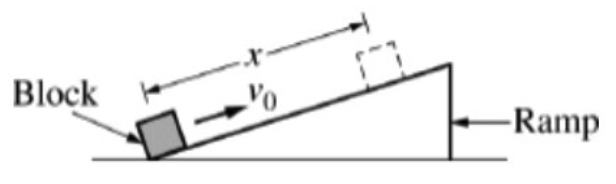
\includegraphics[width=3in]{Screenshot 2022-11-06 at 22.32.47.png}
\end{center}
\begin{enumerate}
    \item Draw two separate FBD representing the box as it slides up the ramp and down the ramp.\\
    \begin{center}\tcbhighmath{
        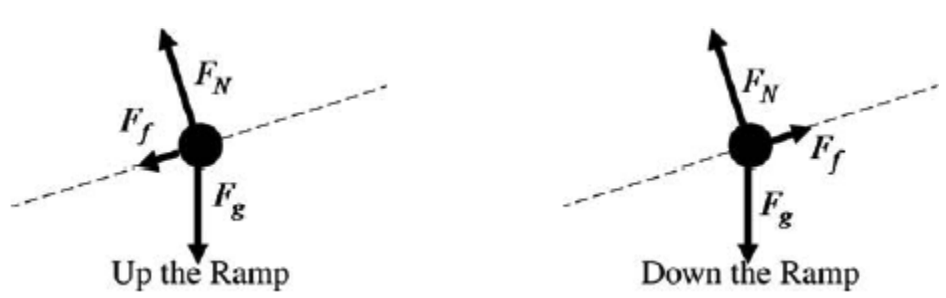
\includegraphics[width=3in]{Screenshot 2022-11-18 at 16.17.28.png} }
    \end{center}
    \item The block takes $t_{\text{up}}$ to slide up the ramp a distance of $x$. The block then takes $t_{\text{down}}$ to slid back down to the bottom of the ramp, where it has a speed $v_f$. Is $t_{\text{down}}$ greater than, equal to, or less than $t_{\text{up}}$?
    In a clear; coherent paragraph-length response that may  contain figures and/or equations; explain your reasoning. Do NOT add anything to the figures in part (a).
    \begin{empheq}[box=\tcbhighmath]{equation*}
        t_{down}>t_{up}
    \end{empheq}
    \begin{empheq}[box=\tcbhighmath]{gather*}
\textbf{1 point is earned: }
  \notag\text{\parbox{.7\linewidth} {For stating that the magnitude of the net force on the block is greater when it is sliding up the ramp than when it is sliding down the ramp because the direction of the frictional force changes while the direction of the component of the gravitational force along the ramp does not.}}\\\\
\textbf{1 point is earned: }
  \notag\text{\parbox{.7\linewidth} {For stating that the magnitude of acceleration of the block while sliding up the ramp is greater than that when sliding down.}}\\\\
  \textbf{1 point is earned: }
  \notag\text{\parbox{.7\linewidth} {For a justification that is $v_f$ less than $v_0$,(e.g., speed changes more on way up than on way down because acceleration is greater on the way up and the same distance covered and final/initial speed on way up/down is zero).}}\\\\
  \textbf{1 point is earned: }
  \notag\text{\parbox{.7\linewidth} {For a correct argument that, if $v_f$ is less than $v_0$ or the average speed up is greater than the average speed down, then $t_{down}$ is greater than $t_{up}$.}}\\\\
    \textbf{1 point is earned: }
  \notag\text{\parbox{.7\linewidth} {For a logical, relevant, and internally consistent argument that addresses the required argument or question asked, and follows the guidelines described in the published requirements for the paragraph-length response.}}
\end{empheq}
\end{enumerate}
\newpage
\item A simple pendulum consists of a bob of mass 1.8kg attached to a string of length 2.3m. The pendulum is held at and angle of $30^{\circ}$ from the vertical by a light horizontal string attached to a wall, as shown below. 

\begin{center}
    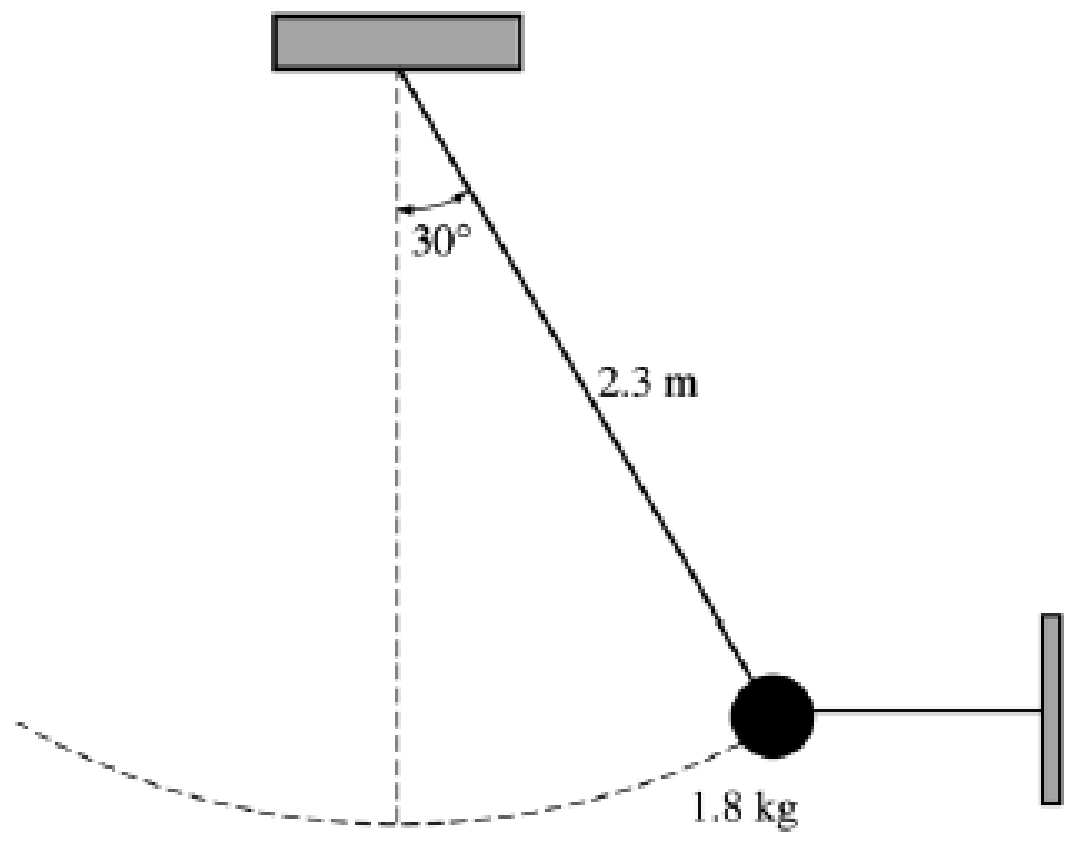
\includegraphics[width=2in]{Screenshot 2022-11-06 at 22.49.38.png}
\end{center}
\begin{enumerate}
    \item  Draw a free-body diagram showing and labelling the forces on the bob in the position shown above.
    \begin{center}\tcbhighmath{
        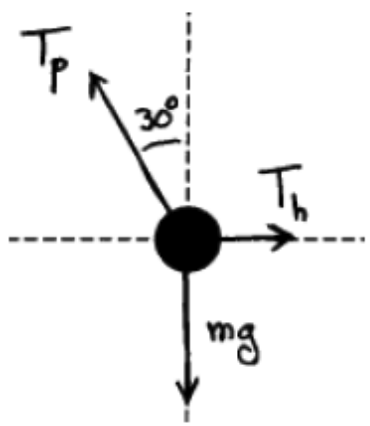
\includegraphics[width=1in]{Screenshot 2022-11-18 at 16.50.57.png}
        }
    \end{center}
    
    \item Calculate the tension in the horizontal string.
    \begin{empheq}[box=\tcbhighmath]{equation*}
        \begin{aligned}
           F_{net_x}= T_P\cos(30^{\circ})-mg = 0 \Longrightarrow T_P = \frac{mg}{\cos(30^{\circ})} = \frac{294\sqrt{3}}{25}\\
           F_{net_y}= T_P\sin(30^{\circ})-T_H = 0 \Longrightarrow T_H=T_P\sin(30^{\circ}) = \frac{147\sqrt{3}}{25}\approx 10.18 N
        \end{aligned}
    \end{empheq}
\end{enumerate}
\newpage
\item
\begin{center}
    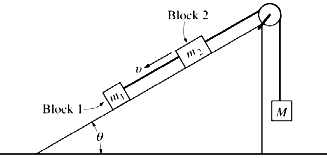
\includegraphics[width=3in]{1.png}
\end{center}
Blocks 1 and 2 of masses $m_1$ and $m_2$,  respectively, are connected by a light string, as shown. These blocks are further connected to a block of mass $M$ by another light string that passes over a pulley of negligible mass and friction. Blocks 1 and 2 move with a constant velocity $v$ down the inclined plane, which makes an angle $\theta$ with the horizontal. The kinetic frictional force on block 1 is $f$ and that on block 2 is $2f$. Express your to questions b-d in terms of $m_1$, $m_2$, $g$, $\theta$, and $f$.
\begin{enumerate}
    \item Draw a free-body diagram showing and labelling the forces of block $m_1$
   \begin{center}\tcbhighmath{
        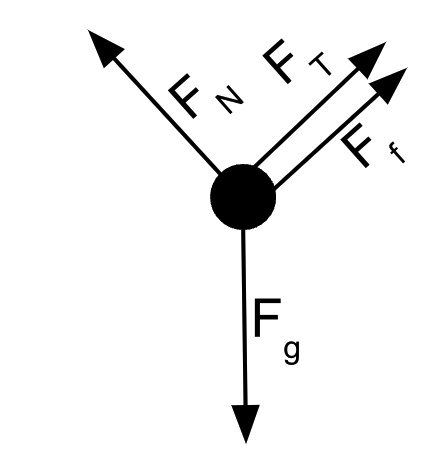
\includegraphics[width=1in]{Screenshot 2022-11-18 at 21.02.29.png}}
    \end{center}
    \item Determine the coefficient of kinetic friction between the inclined plane and block 1.
    \begin{empheq}[box=\tcbhighmath]{equation*}
        \begin{aligned}
           \Sigma F = F_N-F_g_x = 0\\
           F_N=mg\cos(\theta)\\
           F_f=F_N\cdot \mu \Longrightarrow \mu=\frac{F_f}{F_N} = \frac{f}{mg\cos(\theta)}
        \end{aligned}
    \end{empheq}
    \item Determine the value of the suspended mass $M$ that allows blocks 1 and 2 to move with constant velocity down the plane.
    \begin{empheq}[box=\tcbhighmath]{equation*}
        \begin{aligned}
           \Sigma F_{total} = m_{total}a =0\\
            0 = F_g_{x1}+F_g_{x2} - f -2f-F_g_{M}=0\\
            m_1g\sin(\theta)+m_2g\sin(\theta)-3f=Mg\\
            M=\frac{g\sin(\theta)(m_1+m_2)-3f}{g}
        \end{aligned}
    \end{empheq}
    \item The string between blocks 1 and 2 is now cut. Determine the acceleration of block 1 while it is on the inclined plane.
    \begin{empheq}[box=\tcbhighmath]{equation*}
        \begin{aligned}
           \Sigma F_x=m_1 \cdot a_x = F_g_{1x}-F_f = m_1g\sin(\theta)-f\\
           a=g\sin(\theta)-f
        \end{aligned}
    \end{empheq}
\end{enumerate}
\newpage
\item (12 points, suggested time 25 minutes)
\begin{center}
    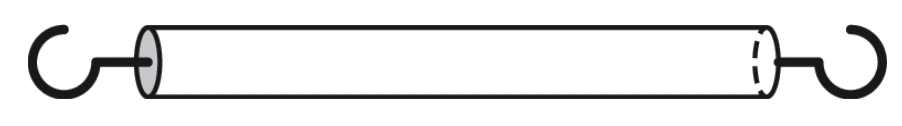
\includegraphics[width=4in]{Screenshot 2022-11-06 at 23.02.56.png}
\end{center}
A group of students is investigating how the thickness of a plastic rod affects the maximum force $F_{\text{max}}$ with which the rod can be pulled without breaking. Two students are discussing models to represent how $F_{\text{max}}$ depends on rod thickness. Student $A$ claims that $F_{\text{max}}$ is directly proportional to the radius of the rod. Student $B$ claims that $F_{\text{max}}$ is directly proportional to the cross-sectional area of the rod—the area of the base of the cylinder, shaded gray in the figure above.
\begin{enumerate}
    \item The students have a collection of many rods of the same material. The rods are all the same length but come in a range of six different thicknesses. Design an experimental procedure to determine which student’s model, if either, correctly represents how $F_{\text{max}}$ depends on rod thickness.\\\\
    In the table below, list the quantities that would be measured in your experiment. Define a symbol to represent each quantity, and also list the equipment that would be used to measure each quantity. You do not need to fill in every row. If you need additional rows, you may add them to the space just below the table. 
\suspend{enumerate}

\begin{table}[h]
\centering
\begin{tabular}{|l|l|l|}
\hline
Quantity to be Measured & Symbol for Quantity & Equipment for Measurement \\ \hline
 &  &  \\ \hline
 &  &  \\ \hline
 &  &  \\ \hline
 &  &  \\ \hline
 &  &  \\ \hline
\end{tabular}
\end{table}

Describe the overall procedure to be used, referring to the table. Provide enough detail so that another student could replicate the experiment, including any steps necessary to reduce experimental uncertainty. As needed, use the symbols defined in the table and/or include a simple diagram of the setup.
\begin{empheq}[box=\tcbhighmath]{gather*}
\textbf{1 point is earned: }
  \notag\text{\parbox{.7\linewidth} {For measuring the radius or diameter of rods with different radii using an appropriate tool.}}\\\\
\textbf{1 point is earned: }
  \notag\text{\parbox{.7\linewidth} {For measuring force using an appropriate tool.}}\\\\
  \textbf{1 point is earned: }
  \notag\text{\parbox{.7\linewidth} {For a plausible/practical way to directly or indirectly determine $F_{max}$ for a given rod.}}\\\\
  \textbf{1 point is earned: }
  \notag\text{\parbox{.7\linewidth} {For attempting to reduce experimental uncertainty in an experiment that involves breaking
the rods.}}\\\\
\end{empheq}
\resume{enumerate}
\newpage
\item For a rod of radius $r_0$, it is determined that $F_{\text{max}}$ is $F_0$, as indicated by the dot on the grid below. On the grid, draw and label graphs corresponding to the two students’ models of the dependence of $F_{\text{max}}$ on rod radius. Clearly label each graph $A$ or $B$, corresponding to the appropriate model.
\begin{center}\tcbhighmath{
    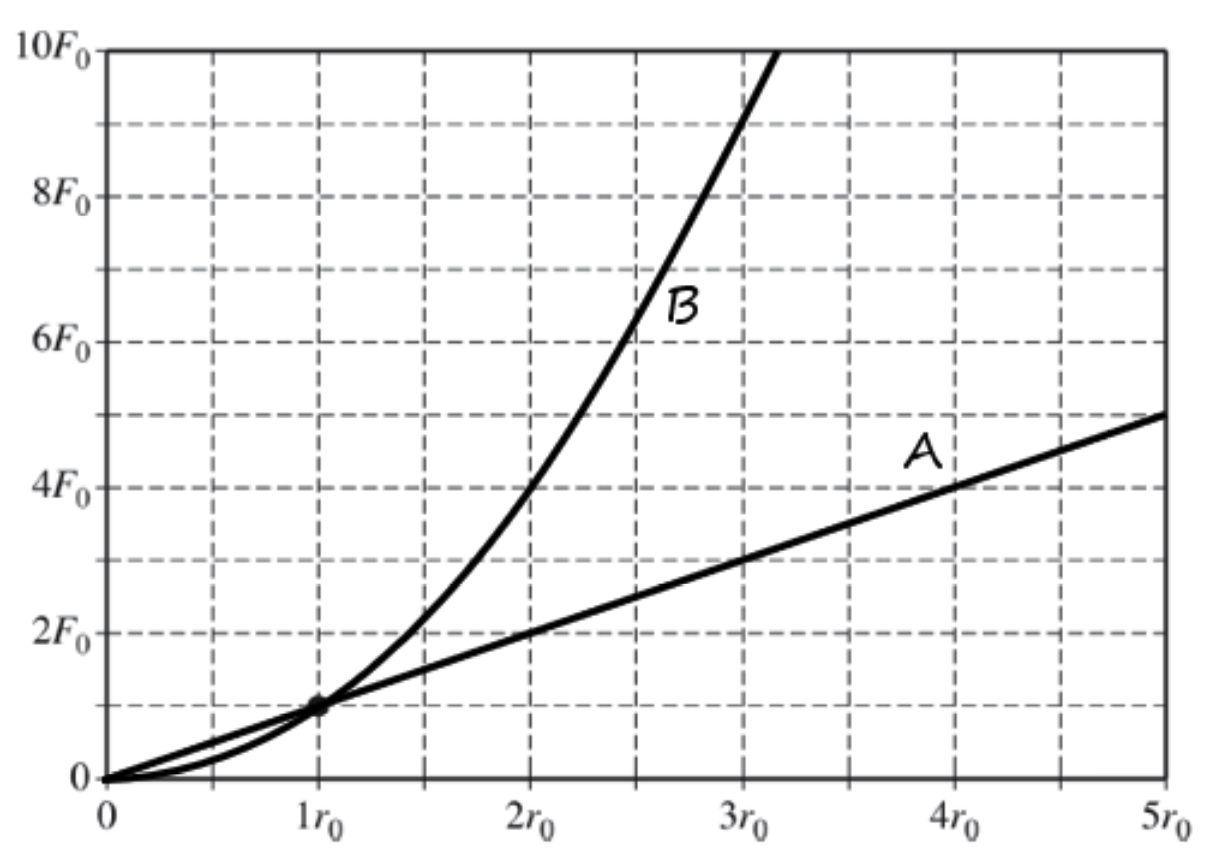
\includegraphics[width=6in]{Screenshot 2022-11-18 at 21.31.45.png}}
\end{center}
\begin{empheq}[box=\tcbhighmath]{gather*}
\textbf{1 point is earned: }
  \notag\text{\parbox{.7\linewidth} {For a straight-line graph marked “A” with a slope of $\frac{F_0}{r_0}$.}}\\\\
  \textbf{1 point is earned: }
  \notag\text{\parbox{.7\linewidth} {For a graph marked “B” that is concave up.}}\\\\
  \textbf{1 point is earned: }
  \notag\text{\parbox{.7\linewidth} {For a graph marked “B” that shows a quadratic relationship at the correct points.}}\\\\
  \textbf{1 point is earned: }
  \notag\text{\parbox{.7\linewidth} {For two graphs that both contain the point $(r_0,F_0)$.}}
\end{empheq}
\end{enumerate}
\newpage
\item The table below shows results of measurements taken by another group of students for rods of different
thicknesses. 

\begin{table}[h]
\centering
\begin{tabular}{|l|l|l|l|l|l|}
\hline
Rod radius (mm) & 0.5 & 1.0 & 1.5 & 2.0 & 2.5 \\ \hline
$F_{\text{max}}$(N) & 40 & 120 & 320 & 520 & 900 \\ \hline
\end{tabular}
\end{table}

Using graph-paper plot the points from the table above. Clearly scale and label all axes, including units. Draw either a straight line or a curve that best represents the data.
\begin{center}\tcbhighmath{
    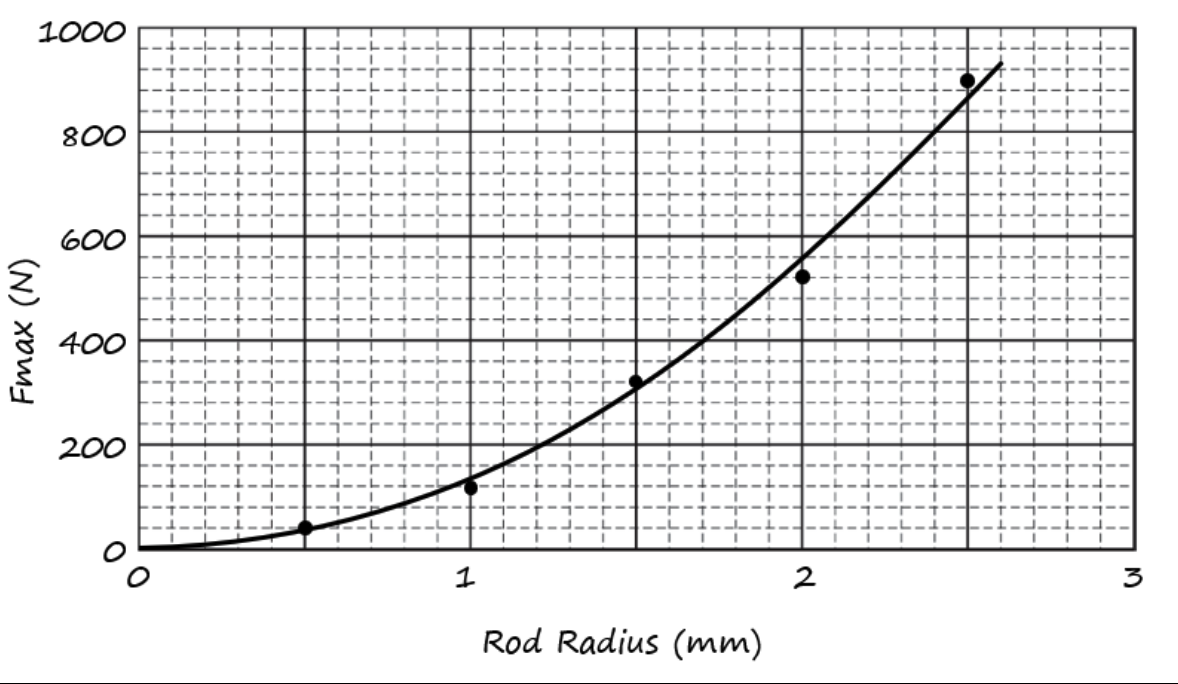
\includegraphics[width=6in]{Screenshot 2022-11-18 at 21.37.17.png}}
\end{center}
\begin{empheq}[box=\tcbhighmath]{gather*}
\textbf{1 point is earned: }
  \notag\text{\parbox{.7\linewidth} {For linear scales with appropriate labels and units \textbf{AND} for a graph where the plotted points cover at least half of the grid’s width and height}}\\\\
  \textbf{1 point is earned: }
  \notag\text{\parbox{.7\linewidth} {For plotting the points correctly.}}\\\\
  \textbf{1 point is earned: }
  \notag\text{\parbox{.7\linewidth} {For drawing a reasonable best-fit curve.}}
\end{empheq}
\item Which student’s model is more closely represented by the evidence shown in the graph you drew in part (c)?\\
\underline{\hspace{1cm}} Student A’s model: $F_{\text{max}}$ is directly proportional to the radius of the rod. \\
\underline{\hspace{1cm}} Student B’s model: $F_{\text{max}}$ is directly proportional to the cross-sectional area of the rod.\\\\ 
Explain your reasoning.
\begin{empheq}[box=\tcbhighmath]{gather*}
\textbf{1 point is earned: }
  \notag\text{\parbox{.7\linewidth} {For identifying Model $B$ and for indicating that $F_{max}$ increases as the square of the radius
increases.}}
\end{empheq}
\end{enumerate}
\newpage
\item (10 points) 
A student of mass $m$ stands on a platform scale in an elevator in a tall building. The positive direction for all vector quantities is upward. 
\begin{enumerate}
    \item Draw a free-body diagram showing and labeling all the forces acting on the student, who is represented by the dot below. 
    \begin{center}\tcbhighmath{
    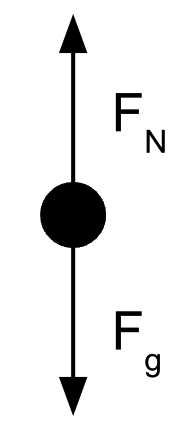
\includegraphics[width=0.5in]{Screenshot 2022-11-18 at 21.44.33.png}}
\end{center}
    \item Derive an expression for the reading on the scale in terms of the acceleration $a$ of the elevator, the mass $m$ of the student, and fundamental constants. 
    \begin{empheq}[box=\tcbhighmath]{equation*}
        \begin{aligned}
           \Sigma F_{net}=ma=F_N-F_g\\
           F_N-mg=ma\\
           F_N=m\cdot(g+a)
        \end{aligned}
    \end{empheq}
\suspend{enumerate}
 An inspector provides the student with the following graph showing the acceleration $a$ of the elevator as a function of time $t$. 
 \begin{center}
     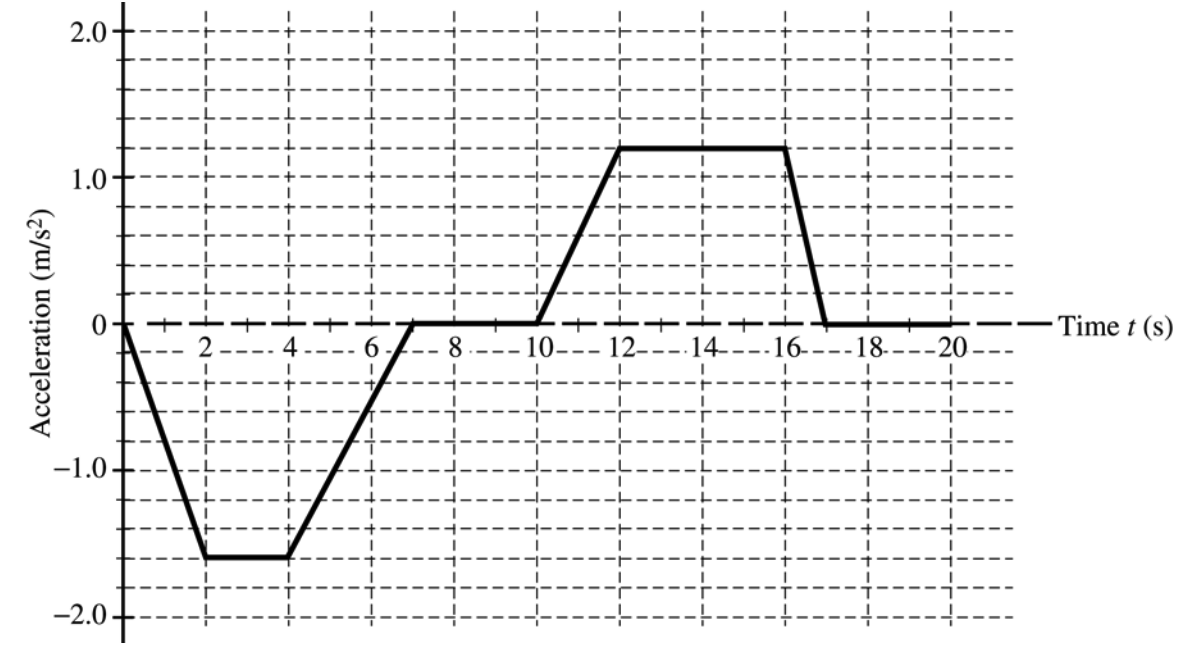
\includegraphics[width=3in]{Screenshot 2022-11-16 at 19.56.16.png}
 \end{center}
\resume{enumerate}
     \item 
     \begin{enumerate}
         \item During what time interval(s) is the force exerted by the platform scale on the student a maximum value?
    \begin{empheq}[box=\tcbhighmath]{equation*}
    \textbf{2 point is earned: }
        \notag\text{\parbox{.7\linewidth}{The normal force exerted by the scale is maximum when the acceleration has its maximum positive value. The force is maximum when $t\in[12s,16s]$}}
    \end{empheq}
        \item Calculate the magnitude of that maximum force for a 45 kg student. 
        \begin{empheq}[box=\tcbhighmath]{equation*}
        \begin{aligned}
           F_N=m\cdot(g+a) = (45kg)(9.8 \frac{m}{s^2}+1.2\frac{m}{s^2})= (45kg)(11.0 \frac{m}{s^2}) = 500N
        \end{aligned}
    \end{empheq}
     \end{enumerate}
     \item During what time interval(s) is the speed of the elevator constant? 
    \begin{empheq}[box=\tcbhighmath]{equation*}
        \textbf{2 point is earned: }
        \notag\text{\parbox{.7\linewidth}{The speed of the elevator is constant when the acceleration is zero.  This occurs when $t\in[7s,10s]$ and $t\in[17s,20s]$ }}
    \end{empheq}
\end{enumerate}
\end{enumerate}
\end{document}